\chapter{الإينولات وأيونات الإينولات والتفاعل الألدولي}\label{ch:b2:enolates-aldol}

في كل مرة تفكك فيها خلية الغلوكوز، يقطع إنزيم فوسفات سكر سداسي الكربون
إلى قطعتين ثلاثيتي الكربون: وهذا تفاعل ألدولي يجري بالعكس. وحين يجري
إلى الأمام، يصل التفاعل نفسه مركبين كربونيليين في مركب واحد، وهو
أكثر طرق الكيميائي استعمالًا لتكوين روابط كربون--كربون. ويقوم على
خاصية لم تمسّها الفصول السابقة إلا مسًّا: فذرات الهيدروجين المجاورة لمجموعة
الكربونيل حمضية، ونزع إحداها يحوّل الكربون المجاور
للكربونيل إلى محب للنواة.

\begin{recall}
مجلد السنة الأولى: $\mathrm pK_a$ والتفاعل الغالب، والأنيونات الكربونية، والتحكم الحركي 
والترموديناميكي، والإضافات المحبة للنواة إلى الكربونيلات، والحذفان E1 وE2، وإماهة
الألكاينات (\omterm{def:b2:enolates-aldol:tautomerism}{إينول} يُعاد ترتيبه). و\cref{ch:b2:frontier-orbitals}: المحبات للنواة الثنائية الموقع.
و\cref{ch:b2:acyl-substitution}: الإسترات والاستبدال الأسيلي.
\end{recall}

\section{تصاوغ الكيتو--الإينول}

\begin{definition}[التصاوغ]\label{def:b2:enolates-aldol:tautomerism}
\emph{المتصاوغات}\index{متصاوغات} متماكبات يتحول بعضها إلى بعض بانتقال هيدروجين ورابطة
مزدوجة. وفي \emph{تصاوغ الكيتو--الإينول}\index{تصاوغ الكيتو--الإينول}، يكون المركب الكربونيلي الحامل
لهيدروجين على الكربون المجاور للكربونيل (صورة الكيتو) في توازن مع
\emph{إينوله}\index{إينول}، وهو كحول تحمله رابطة مزدوجة \ce{C=C}.
\end{definition}

\begin{omfigure}
\setchemfig{atom sep=2em}
\schemestart
\chemfig{H_3C-C(=[2]O)-CH_3}
\arrow{<=>[\ce{H+} أو \ce{HO-}][حفز]}[,2.2]
\chemfig{H_3C-C(-[2]OH)=CH_2}
\schemestop
\par\vspace{6pt}

{\small البروبانون \omterm{def:b2:enolates-aldol:tautomerism}{وإينوله}، البروب-1-ين-2-ول. يحفز التحول بينهما الحمض (برتنة أكسجين الكربونيل، ثم فقد
هيدروجين $\alpha$) أو القاعدة (نزع هيدروجين $\alpha$، ثم برتنة الأكسجين)؛
ويقع التوازن بعيدًا في جهة صورة الكيتو.}
\end{omfigure}

\begin{proposition}[محتوى الإينول]\label{prop:b2:enolates-aldol:enol-content}
لا تحوي الألدهيدات والكيتونات البسيطة إلا آثارًا من \omterm{def:b2:enolates-aldol:tautomerism}{الإينول}؛ أما المركبات 1،3-ثنائية الكربونيل مثل
البنتان-2،4-ديون فتحوي نسبة كبيرة منه.
\end{proposition}

\begin{proof}[تعليل]
الرابطة \ce{C=O} أقوى من الرابطة \ce{C=C} بأكثر مما تضعف الرابطة \ce{O-H} عن الرابطة \ce{C-H}:
فتُفضَّل صورة الكيتو. وفي المركب 1،3-ثنائي الكربونيل، تترافق الرابطة المزدوجة \omterm{def:b2:enolates-aldol:tautomerism}{للإينول}
مع مجموعة الكربونيل الثانية، وتكوّن \ce{OH} \omterm{def:b2:enolates-aldol:tautomerism}{الإينول} رابطة هيدروجينية داخلية مع أكسجينها
في حلقة سداسية: وكلا الأمرين يثبّت \omterm{def:b2:enolates-aldol:tautomerism}{الإينول} بما يكفي لجعله صورة رئيسية.
\end{proof}

ولأن \omterm{def:b2:enolates-aldol:tautomerism}{الإينول} مستوٍ عند رابطته \ce{C=C}، يضيع المركز الفراغي عند الكربون $\alpha$ في كل مرة
يتكوّن فيها \omterm{def:b2:enolates-aldol:tautomerism}{الإينول}: فالكيتون النشط ضوئيًا ذو المركز الفراغي المجاور لكربونيله يتحول إلى راسيمي في الحمض
أو القاعدة.

\section{أيونات الإينولات}

\begin{definition}[أيونات الإينولات]\label{def:b2:enolates-aldol:enolate}
\emph{الكربون $\alpha$}\index{كربون ألفا@كربون $\alpha$} لمركب كربونيلي هو الكربون
المرتبط بكربون الكربونيل؛ وهيدروجيناته هي \emph{هيدروجينات $\alpha$}\index{هيدروجين ألفا@هيدروجين $\alpha$}.
ونزع أحدها يعطي \emph{أيون الإينولات}\index{أيون الإينولات}، الذي تتوزع
شحنته السالبة بين الكربون $\alpha$ والأكسجين.
\end{definition}

\begin{proposition}[حموضة هيدروجينات $\alpha$]\label{prop:b2:enolates-aldol:alpha-acidity}
هيدروجينات $\alpha$ أكثر حموضة بكثير من روابط \ce{C-H} العادية لأن \omterm{def:b2:enolates-aldol:enolate}{أيون الإينولات} يثبّته
الرنين؛ والهيدروجين الواقع بين مجموعتي كربونيل حمضي بما يكفي لينزعه ألكوكسيد أو
حتى هيدروكسيد.
\end{proposition}

\begin{proof}[تعليل]
في \omterm{def:b2:enolates-aldol:enolate}{أيون الإينولات} تقع الشحنة السالبة جزئيًا على الأكسجين الكهرسلبي؛ وكربونيل ثانٍ في
الجهة الأخرى يجعلها غير متمركزة على أكسجينين. ومقيسًا في الماء، للبنتان-2،4-ديون $\mathrm pK_a =
9.0$ وللإستر 3-أوكسوبيوتانوات الإيثيل 10.7، وهما قيمتان تقارنان بقيمة النتروميثان (10.2)، الذي يثبّت أنيونَه
مجموعةُ النترو بالطريقة نفسها؛ أما الكيتون البسيط، بكربونيله الوحيد، فأضعف بكثير --- أضعف من
أن تُقاس حموضته مباشرة في الماء.
% ledger: pka:acac, pka:acetoacetate, pka:nitromethane
\end{proof}

\begin{omfigure}
\setchemfig{atom sep=2em}
\schemestart
\chemfig{H_3C-C(=[2]O)-\chemabove{C}{\scriptstyle -}H_2}
\arrow{<->}
\chemfig{H_3C-C(-[2]\chemabove{O}{\scriptstyle -})=CH_2}
\schemestop
\par\vspace{6pt}

{\small بنيتا الرنين لأيون إينولات البروبانون. تتقاسم الشحنة السالبة
الكربونُ $\alpha$ والأكسجين: \omterm{def:b2:enolates-aldol:enolate}{فأيون الإينولات} \omterm{def:b2:frontier-orbitals:ambident}{محب للنواة ثنائي الموقع}، يتفاعل مع معظم المحبات للإلكترونات
الكربونية عند الكربون.}
\end{omfigure}

\begin{definition}[الإينولات الحركي والإينولات الترموديناميكي]\label{def:b2:enolates-aldol:kinetic-enolate}
في كيتون ذي كربونين $\alpha$ مختلفين، يكون \emph{الإينولات الحركي}\index{إينولات حركي}
هو المتكوّن أسرع، بنزع هيدروجين من الجهة الأقل إعاقة والأقل استبدالًا؛ ويكون
\emph{الإينولات الترموديناميكي}\index{إينولات ترموديناميكي} هو الأكثر استقرارًا، ذا الرابطة المزدوجة
الأكثر استبدالًا.
\end{definition}

\begin{proposition}[اختيار الإينولات]\label{prop:b2:enolates-aldol:enolate-control}
القاعدة القوية الضخمة المستعملة بكمية كاملة في درجة حرارة منخفضة (ثنائي إيزوبروبيل أميد الليثيوم، LDA، عند
\qty{-78}{\degreeCelsius}) تكوّن \omterm{def:b2:enolates-aldol:kinetic-enolate}{الإينولات الحركي} كليًا وبلا رجعة؛ أما القاعدة الأضعف في درجة حرارة
الغرفة (ألكوكسيد في كحوله) فتسمح للإينولات بالتحول بعضها إلى بعض وتعطي في معظمها
\omterm{def:b2:enolates-aldol:kinetic-enolate}{الإينولات الترموديناميكي}.
\end{proposition}

\begin{proof}[تعليل]
LDA (و$\mathrm pK_a$ لثنائي إيزوبروبيل أمين نحو 36، أعلى بكثير من قيمة الكيتون) تنزع البروتون كليًا 
وبسرعة؛ وفي درجة الحرارة المنخفضة لا يُعاد برتنة الإينولات، فيحسم الأمرَ نزعُ البروتون الأسرع، عند
\ce{CH2} أو \ce{CH3} الأسهل منالًا: تحكم حركي. أما الألكوكسيد فلا ينزع البروتون إلا جزئيًا،
وتتبادل الإينولات والكيتون البروتونات باستمرار، ويحابي خليط التوازن الإينولات
الأكثر استبدالًا والأكثر استقرارًا: تحكم ترموديناميكي (كما في مجلد السنة الأولى).
% ledger: ghs:LDA
\end{proof}

\section{ألكلة أيونات الإينولات}

تهاجم أيونات الإينولات الألكانات المهلجنة الأولية باستبدال ثنائي الجزيئية، فتكوّن رابطة \ce{C-C} جديدة عند
الكربون $\alpha$. ومع هيدروجينات $\alpha$ الشديدة الحموضة في المركب 1،3-ثنائي الكربونيل، يكفي
ألكوكسيد، ويمكن إزالة الكربونيل الإضافي بعد ذلك.

\begin{definition}[نزع الكربوكسيل]\label{def:b2:enolates-aldol:decarboxylation}
\emph{نزع الكربوكسيل}\index{نزع الكربوكسيل} يزيل مجموعة كربوكسيل على هيئة \ce{CO2}. وفي
\emph{تخليق إستر المالونيك}\index{تخليق إستر المالونيك}، يُنزع بروتون من بروبانديوات ثنائي الإيثيل،
ويُؤلكَل، ويُحلمَه إلى حمض البروبانديويك المستبدَل ثم يُنزع منه الكربوكسيل بالتسخين، فيعطي
حمضًا كربوكسيليًا \ce{RCH2COOH}.
\end{definition}

\begin{proposition}[نزع كربوكسيل سهل]\label{prop:b2:enolates-aldol:decarboxylation}
الأحماض $\beta$-الكيتونية وأحماض البروبانديويك تفقد \ce{CO2} بالتسخين اللطيف؛ أما الأحماض الكربوكسيلية العادية
فلا.
\end{proposition}

\begin{proof}[تعليل]
الكربونيل البعيد رابطتين عن مجموعة الكربوكسيل يستقبل هيدروجين \ce{COOH} في حالة انتقالية
حلقية سداسية بينما يغادر \ce{CO2}: فيتكوّن \omterm{def:b2:enolates-aldol:tautomerism}{إينول} مباشرة، ثم يتصاوغ. ودون
ذلك الكربونيل، لا يجد الأنيون الكربوني الذي يخلّفه فقد \ce{CO2} أي تثبيت.
\end{proof}

\begin{definition}[تفاعل الهالوفورم]\label{def:b2:enolates-aldol:haloform}
\emph{تفاعل الهالوفورم}\index{تفاعل الهالوفورم} يحوّل ميثيل كيتونًا \ce{RCOCH3}، بوجود
هالوجين وفائض من الهيدروكسيد، إلى كربوكسيلات \ce{RCOO-} وهالوفورم \ce{CHX3}.
\end{definition}

كل هالوجين يدخل يجعل هيدروجينات $\alpha$ المتبقية أكثر حموضة، فتُهلجن مجموعة الميثيل
ثلاث مرات؛ ثم تصير المجموعة \ce{CX3-} مجموعة مغادرة جيدة بما يكفي ليطردها الهيدروكسيد في
استبدال أسيلي. ومع اليود، يكون الراسب الأصفر لليودوفورم كشفًا عن ميثيل الكيتونات.

\section{التفاعل الألدولي}

\begin{definition}[التفاعلات الألدولية]\label{def:b2:enolates-aldol:aldol}
في \emph{الإضافة الألدولية}\index{إضافة ألدولية} يُضاف \omterm{def:b2:enolates-aldol:enolate}{أيون الإينولات} (أو \omterm{def:b2:enolates-aldol:tautomerism}{الإينول}) لمركب كربونيلي
إلى مجموعة الكربونيل لمركب آخر، فيعطي مركبًا كربونيليًا $\beta$-هيدروكسيليًا، هو
\emph{الألدول}\index{ألدول}. وفي \emph{التكاثف الألدولي}\index{تكاثف ألدولي} يفقد الألدول
الماء، فيعطي مركبًا كربونيليًا $\alpha,\beta$-غير مشبع (إينون أو إينال).
\end{definition}

\begin{omfigure}
\setchemfig{atom sep=1.9em}
\schemestart
\chemfig{H_3C-CH=O} \+ \chemfig{^{-}CH_2-CH=O}
\arrow{->[إضافة]}
\chemfig{H_3C-CH(-[2]O^{-})-CH_2-CH=O}
\schemestop

\medskip
\schemestart
\arrow{->[\ce{H2O}][$-$ \ce{HO-}]}
\chemfig{H_3C-CH(-[2]OH)-CH_2-CH=O}
\arrow{->[تسخين، قاعدة][$-$ \ce{H2O}]}
\chemfig{H_3C-CH=CH-CH=O}
\schemestop
\par\vspace{6pt}

{\small التفاعل الألدولي للإيثانال. يُضاف \omterm{def:b2:enolates-aldol:enolate}{أيون الإينولات} إلى جزيء ثانٍ من الإيثانال؛ وتعطي البرتنة
\omterm{def:b2:enolates-aldol:aldol}{الألدول}، 3-هيدروكسي بيوتانال. وبالتسخين مع قاعدة، يُنزع هيدروجين $\alpha$ ويغادر الهيدروكسيد
من الكربون $\beta$: البوت-2-ينال، المترافق.}
\end{omfigure}

\begin{proposition}[دفع التفاعل الألدولي]\label{prop:b2:enolates-aldol:aldol-equilibrium}
\omterm{def:b2:enolates-aldol:aldol}{الإضافة الألدولية} عكوسة؛ ونزع الماء، الذي يكوّن نظامًا مترافقًا، يسحب
التفاعل نحو ناتج التكاثف.
\end{proposition}

\begin{proof}[تعليل]
جزيئان يعطيان جزيئًا واحدًا، فتكون \omterm{def:b2:reaction-free-energy:reaction-entropy}{إنتروبيا التفاعل} سالبة، والرابطة \ce{C-C} الجديدة بالكاد
تعوّض رابطة $\pi$ المفقودة في \ce{C=O}: فلكثير من الكيتونات يكون $K$ صغيرًا. وإزالة \omterm{def:b2:enolates-aldol:aldol}{الألدول} بنزع الماء
تُبقي $Q < K$ للإضافة؛ والإينون المترافق المتكوّن مستقر، وفي درجة الحرارة المرتفعة،
يحابيه ربح الإنتروبيا الناتج عن تحرير الماء أكثر. والتفاعل العكسي، الألدولي العكسي، هو
الخطوة التي تشطر بها الخلية سكرًا سداسي الكربون.
\end{proof}

\begin{method}[التحكم في تفاعل ألدولي متصالب]\label{met:b2:enolates-aldol:crossed-aldol}
\begin{enumerate}
  \item استعمل شريكًا بلا هيدروجينات $\alpha$ (البنزالدهيد، الميثانال): فلا يكون إلا
        المحب للإلكترونات.
  \item أو كوّن أيون إينولات أحد الشريكين كليًا أولًا (LDA، \qty{-78}{\degreeCelsius})، ثم أضف
        الآخر.
  \item أو استعمل شريكًا 1،3-ثنائي الكربونيل، أكثر حموضة بكثير من الآخر.
  \item فضّل ألدهيدًا محبًا للإلكترونات: فهو أكثر تفاعلية من الكيتون.
\end{enumerate}
\end{method}

\begin{method}[التعرف على ناتج ألدولي]\label{met:b2:enolates-aldol:aldol-recognition}
\begin{enumerate}
  \item ابحث عن \ce{C=O} مع \ce{OH} على الكربون البعيد ذرتين ($\beta$)، أو عن \ce{C=C}
        مترافقة مع \ce{C=O}.
  \item اقطع الرابطة بين الكربونين $\alpha$ و$\beta$: كان الكربون $\beta$ كربون كربونيل (المحب
        للإلكترونات)، والكربون $\alpha$ كربون \omterm{def:b2:enolates-aldol:enolate}{أيون الإينولات}.
  \item تحقق من وجود الشريكين ومن إمكان تكوين \omterm{def:b2:enolates-aldol:enolate}{أيون الإينولات} انتقائيًا.
\end{enumerate}
\end{method}

\section{تكاثف كلايزن}

\begin{definition}[تكاثف كلايزن]\label{def:b2:enolates-aldol:claisen}
في \emph{تكاثف كلايزن}\index{تكاثف كلايزن}، يهاجم أيون إينولات إستر
كربونيل جزيء إستر آخر في استبدال أسيلي، فيعطي \emph{إسترًا $\beta$-كيتونيًا}\index{إستر بيتا-كيتوني@إستر $\beta$-كيتوني}
ويحرر ألكوكسيدًا. ونسخته الداخلية الجزيئية، حلقنة ديكمان،
تعطي إسترًا $\beta$-كيتونيًا حلقيًا.
\end{definition}

\begin{proposition}[ما يدفع تكاثف كلايزن]\label{prop:b2:enolates-aldol:claisen-drive}
يحتاج \omterm{def:b2:enolates-aldol:claisen}{تكاثف كلايزن} لإيثانوات الإيثيل إلى مكافئ كامل من إيثوكسيد الصوديوم: فتوازنه
غير مواتٍ، ويدفعه نزع البروتون من الإستر $\beta$-الكيتوني المتكوّن.
\end{proposition}

\begin{proof}
للتكاثف بذاته، \ce{2CH3COOEt <=> CH3COCH2COOEt + EtOH}، ثابت توازن صغير
$K_1$. ثم يُنزع البروتون من الإستر $\beta$-الكيتوني ($\mathrm pK_a = 10.7$) بالإيثوكسيد (الإيثانول، 15.9):
$K_2 = 10^{15.9 - 10.7} = 10^{5.2}$. وللتفاعل الإجمالي، التكاثف مع نزع البروتون، الثابت
$K_1K_2$، الكبير بما يكفي حتى مع $K_1$ صغير؛ فتُستهلك القاعدة وتعطي المعالجة الحمضية الإستر
$\beta$-الكيتوني المتعادل. والإستر الذي ليس له إلا هيدروجين $\alpha$ واحد، والذي لا يمكن نزع بروتون ناتجه، يعطي
ناتجًا قليلًا.
% ledger: pka:acetoacetate, pka:ethanol
\end{proof}

\begin{history}[الألدول، 1872]
\begin{minipage}[t]{0.18\linewidth}
\vspace{0pt}
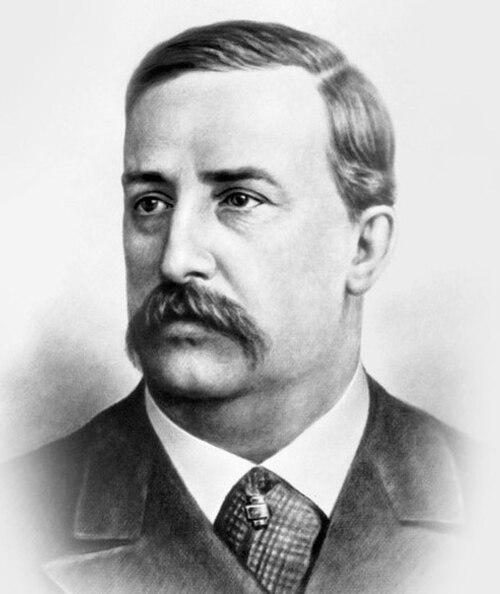
\includegraphics[width=\linewidth]{images/book3/borodin.jpg}
\end{minipage}\hspace{0.02\linewidth}%
\begin{minipage}[t]{0.18\linewidth}
\vspace{0pt}
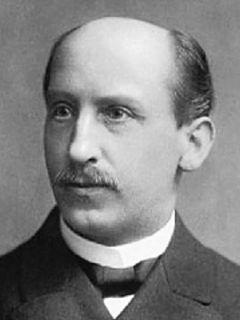
\includegraphics[width=\linewidth]{images/book3/claisen.jpg}
\end{minipage}\hfill
\begin{minipage}[t]{0.58\linewidth}
\vspace{0pt}
وصف التفاعلَ الألدولي سنة 1872 شارل-أدولف فورتز، ومستقلًا عنه ألكسندر
بورودين، الكيميائي في سانت بطرسبورغ، المعروف اليوم أكثر بوصفه مؤلف أوبرا \textit{«الأمير إيغور»}.
ووسّع لودفيغ كلايزن تكاثفات المركبات الكربونيلية لتشمل الإسترات سنة 1887. (صورتان شخصيتان: بورودين،
مؤلف مجهول، ملكية عامة؛ وكلايزن، بعدسة فيرونيكا فيلاغراسا، CC~BY-SA~4.0؛ ويكيميديا كومنز.)
\end{minipage}
\end{history}

\begin{safety}{\ghs[5mm]{GHS02}\,\ghs[5mm]{GHS05}\,\ghs[5mm]{GHS07}}
إيثوكسيد الصوديوم وثنائي إيزوبروبيل أميد الليثيوم أكّالان ويتفاعلان مع الماء؛ ومحاليل LDA
قابلة للاشتعال وتُتداول تحت غاز خامل. والبنزالدهيد والبروبانون ضاران وقابلان للاشتعال.
% ledger: ghs:NaOEt, ghs:LDA, ghs:benzaldehyde, ghs:acetone
\end{safety}

\section{تمارين}

\begin{exercise}[$\star$]\label{exo:b2:enolates-aldol:1}
ارسم \omterm{def:b2:enolates-aldol:tautomerism}{المتصاوغات} الإينولية للبيوتانون وللهكسانون الحلقي.
\end{exercise}

\begin{exercise}[$\star$]\label{exo:b2:enolates-aldol:2}
رتّب بحسب حموضة أكثر روابط \ce{C-H} حموضة فيها: البروبانون، والبنتان-2،4-ديون، و3-أوكسوبيوتانوات الإيثيل،
والإيثان.
\end{exercise}

\begin{exercise}[$\star$]\label{exo:b2:enolates-aldol:3}
أعطِ \omterm{def:b2:enolates-aldol:aldol}{الألدول} وناتج التكاثف للإيثانال مع هيدروكسيد الصوديوم.
\end{exercise}

\begin{exercise}[$\star$]\label{exo:b2:enolates-aldol:4}
اكتب \omterm{def:b2:enolates-aldol:decarboxylation}{تخليق إستر المالونيك} لحمض الهكسانويك: ما الألكان المهلجن اللازم؟
\end{exercise}

\begin{exercise}[$\star\star$]\label{exo:b2:enolates-aldol:5}
ارسم أيوني \omterm{def:b2:enolates-aldol:kinetic-enolate}{الإينولات الحركي} والترموديناميكي للمركب 2-ميثيل هكسانون حلقي والظروف التي تعطي
كلًّا منهما.
\end{exercise}

\begin{exercise}[$\star\star$]\label{exo:b2:enolates-aldol:6}
أعطِ ناتج \omterm{def:b2:enolates-aldol:aldol}{التكاثف الألدولي} المتصالب للبنزالدهيد مع البروبانون (مكافئ واحد من كل
منهما) وفسّر لماذا لا يتكاثف البنزالدهيد مع نفسه.
\end{exercise}

\begin{exercise}[$\star\star$]\label{exo:b2:enolates-aldol:7}
يخضع الهكسان-2،5-ديون في القاعدة \omterm{def:b2:enolates-aldol:aldol}{لتكاثف ألدولي} داخلي الجزيء. أي حلقة تتكوّن؟ فسّر
الاختيار بين الحلقات الممكنة.
\end{exercise}

\begin{exercise}[$\star\star$]\label{exo:b2:enolates-aldol:8}
اكتب \omterm{def:b2:enolates-aldol:claisen}{تكاثف كلايزن} لإيثانوات الإيثيل وناتجه بعد المعالجة الحمضية.
\end{exercise}

\begin{exercise}[$\star\star$]\label{exo:b2:enolates-aldol:9}
أي هذه المركبات يعطي كشف اليودوفورم موجبًا: البروبانون، البنتان-3-ون، الإيثانال، الأسيتوفينون؟
\end{exercise}

\begin{exercise}[$\star\star\star$]\label{exo:b2:enolates-aldol:10}
اكتب حلقنة ديكمان لهكسانديوات ثنائي الإيثيل وحجم حلقة الناتج.
\end{exercise}

\begin{exercise}[$\star\star\star$]\label{exo:b2:enolates-aldol:11}
يفقد (\textit{R})-3-ميثيل بنتان-2-ون نشاطه الضوئي في هيدروكسيد الصوديوم المخفف، لكن
(\textit{R})-4-ميثيل هكسان-2-ون لا يفقده. فسّر.
\end{exercise}

\begin{exercise}[$\star\star\star$]\label{exo:b2:enolates-aldol:12}
اقترح طريقًا إلى 1،5-ثنائي فينيل بنتا-1،4-دين-3-ون، ثم إلى دينون بمجموعتي أريل مختلفتين،
وقل لماذا يكون الثاني أصعب.
\end{exercise}

\section{مسألة: ثنائي بنزال الأسيتون}

\begin{problem}[{مسألة نهاية الأسبوع --- أيون إينولات البروبانون ودور البنزالدهيد، والتكاثفان
الألدوليان، والناتج المترافق، وقياسات الكميات ومردود التحضير}]
\label{pb:b2:enolates-aldol:1}
التحضير (معطيات تمرين): يُحرَّك \qty{2.1}{mL} من البنزالدهيد و\qty{0.75}{mL} من البروبانون
في الإيثانول مع هيدروكسيد الصوديوم المائي؛ فتنفصل بلورات صفراء من 1،5-ثنائي فينيل بنتا-1،4-دين-3-ون
(ثنائي بنزال الأسيتون)؛ والمردود 75~\%. والكثافات (\unit{g/cm^3}): البنزالدهيد 1.045، والبروبانون 0.7845.
والكتل المولية (\unit{g/mol}): C 12.011، H 1.008، O 15.999.
% ledger: rho:benzaldehyde, rho:acetone, aw:C, aw:H, aw:O, ghs:dibenzalacetone

\medskip
\noindent\textbf{الجزء الأول --- الشريكان.}
\begin{enumerate}
  \item أي الشريكين له هيدروجينات $\alpha$؟ وكم عددها؟
  \item ارسم أيون إينولات البروبانون.
  \item لماذا لا يستطيع البنزالدهيد تكوين أيون إينولات؟
  \item لماذا يتفاعل البروبانون مع البنزالدهيد لا مع نفسه؟
  \item لماذا يكون الألدهيد محبًا للإلكترونات أفضل من الكيتون؟
  \item لماذا يكفي الهيدروكسيد قاعدةً هنا؟
\end{enumerate}

\medskip
\noindent\textbf{الجزء الثاني --- الآلية.}
\begin{enumerate}[resume]
  \item اكتب إضافة \omterm{def:b2:enolates-aldol:enolate}{أيون الإينولات} إلى البنزالدهيد.
  \item اكتب نزع الماء من \omterm{def:b2:enolates-aldol:aldol}{الألدول} المتكوّن.
  \item لماذا يكون نزع الماء سهلًا هنا؟
  \item لماذا يمكن أن يحدث التفاعل مرة ثانية؟
  \item اكتب المعادلة الإجمالية.
  \item ما الذي يدفع التفاعل إلى نهايته في هذا التحضير؟
\end{enumerate}

\medskip
\noindent\textbf{الجزء الثالث --- الناتج.}
\begin{enumerate}[resume]
  \item كم رابطة مزدوجة \ce{C=C} لثنائي بنزال الأسيتون، وما ترتيبها الفراغي (في الغالب)؟
  \item لماذا يُفضَّل المتماكب (\textit{E}،\textit{E})؟
  \item عُدّ روابط $\pi$ المترافقة.
  \item لماذا يكون المركب أصفر بينما شريكاه عديما اللون؟
  \item هل ثنائي بنزال الأسيتون كيرالي؟
\end{enumerate}

\medskip
\noindent\textbf{الجزء الرابع --- قياسات الكميات والمردود.}
\begin{enumerate}[resume]
  \item احسب الكتل المولية للبنزالدهيد والبروبانون وثنائي بنزال الأسيتون.
  \item احسب كميتي الكاشفين.
  \item أي الكاشفين محدد؟
  \item احسب الكتلة النظرية للناتج.
  \item لماذا يُفضَّل فائض طفيف من البنزالدهيد على فائض من البروبانون؟
  \item ماذا يعطي فائض من البروبانون؟
  \item اذكر كتلة ثنائي بنزال الأسيتون الناتجة بمردود 75~\%.
\end{enumerate}
\end{problem}
